\chapter{Background}

\section{The Maritime Connectivity Platform}
The Maritime Connectivity Platform (MCP), which is formally known as the Maritime Cloud is a platform, developed by EfficienSea2 \cite{efficienSea2}, which is led by the Danish Maritime Consortium. MCP is a communication framework, that is to ensure efficient, reliable and secure communication, and exchange of information in the maritime sector.
The goal of the platform is to connect maritime stakeholders with maritime information services.
\begin{figure}[H]
	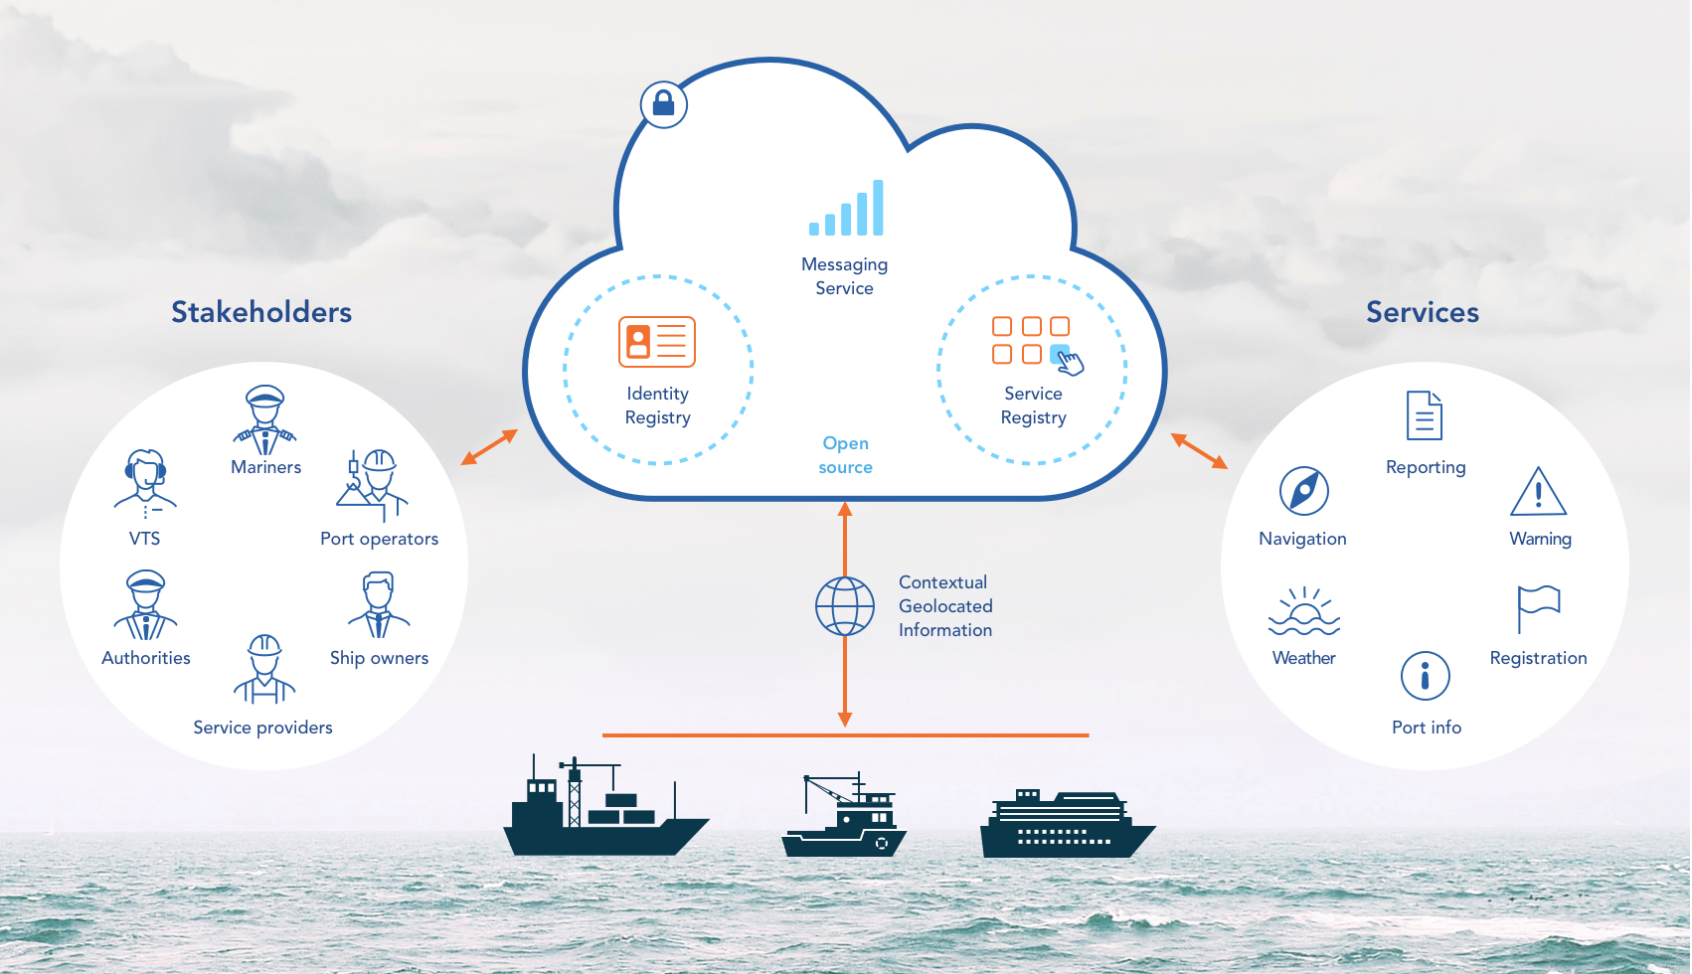
\includegraphics[width=1\textwidth]{figures/MCPStructure}
	\caption{Diagram, describing the structure of MCP \cite{efficienSea2}}
	\label{fig:MCPStruct}
\end{figure}\noindent
A high-level diagram, describing the structure of the MCP can be seen in Figure \ref{fig:MCPStruct}. Here it is shown that maritime stakeholders are connected with the maritime services through the Identity Registry, the Service Registry and the Messaging Service.

\subsection{Identity Registry}
Here the relevant information regarding maritime stakeholders are stored. This information needs to be authorized and stored at a safe location in order for the security of the MCP to be sufficient. The Identity Registry on the MCP is equivalent to the Central Person Registry of a country. The Identity Registry is vital to the MCP in it ensures the solution's authenticity, integrity, and confidentiality. Maritime stakeholders are, through the Identity Registry provided with a single login to all Maritime Services.\cite{efficienSea2}
\subsection{Service Registry}
The Service Registry acts to Maritime Services as the Identity Registry acts to the Maritime Stakeholders. Here all Maritime Services are registered and stored. The Service Registry holds both commercial and non-commercial, as well as authorized and non-authorized services, either free of charge or for a fee. The Service Registry is comparable with the App Store or Google Play in that it distributes services of all kinds to registered users.\cite{efficienSea2}
\subsection{Messaging Service}
\tit{"An information broker that intelligently exchanges information between communication systems connected to the platform, taking into account the current geographical position and communication links available to the recipient."}\cite{efficienSea2}
\section{Model-Based Testing}

\section{Automated Model-Based testing of MCP}